 \documentclass[t]{beamer}
%\documentclass[c]{beamer}
\listfiles

\mode<presentation>
{
  \usetheme[english,titlepage0]{KIT}
% \usetheme[usefoot]{KIT}
% \usetheme{KIT}

%%  \usefonttheme{structurebold}

  \setbeamercovered{transparent}

  %\setbeamertemplate{enumerate items}[circle]
  \setbeamertemplate{enumerate items}[ball]

}
\usepackage{babel}
%\date{10.05.2010}
%\DateText

\newlength{\Ku}
\setlength{\Ku}{1.43375pt}

\usepackage[latin1]{inputenc}
\usepackage[TS1,T1]{fontenc}
\usepackage{array}
\usepackage{multicol}
\usepackage{lipsum}

\usetikzlibrary{shadows,arrows,positioning,matrix,calc}
\definecolor{kit}{RGB}{0,150,130}
\definecolor{kitblue}{RGB}{73,48,164}
\definecolor{firmred}{RGB}{255,153,153}
\definecolor{firmblue}{RGB}{162,153,246}
\definecolor{firmgreen}{RGB}{153,255,153}
\definecolor{grey}{RGB}{130,130,130}
\tikzset{
	cfn/.style={
		draw,rectangle
	},
	cond/.style={
		fill=firmred
	},
	phi/.style={
		fill=firmgreen
	},
	cf/.style={
		color=firmblue,
		line width=1pt,
	},
	cfb/.style={
		color=firmblue,
		line width=2pt,
	},
	asslabel/.style={
		rectangle,
		text width=1.5cm,
		align=left
	},
	ass/.style={
		rectangle,
		text width=3cm,
		align=left
	},
	assline/.style={
		color=grey,
		align=right
	},
	reglifetime/.style={
		-,
		line width=0.5mm,
		draw=kit
	},
	helplinegrey/.style={
		color=grey
	},
	resultregister/.style={ },
	graphnode/.style={
		circle,
		draw=black
	},
	colorbox/.style={
		minimum width=4mm,
		minimum height=4mm,
	},
}

%\usenavigationsymbols
%\usenavigationsymbols[sfHhdb]
%\usenavigationsymbols[sfhHb]

\title[]{Compiler: Assembler generation}
%\subtitle{Karlsruhe Institute of Technology (KIT)}

\author[]{KIT}

\AuthorTitleSep{\relax}

\institute[]{KARLSRUHE INSTITUTE OF TECHNOLOGY (KIT)}
%\institute[\raisebox{-4mm}{\includegraphics[height=5mm]{images/OU-Logo}}]
%  {KARLSRUHE INSTITUTE OF TECHNOLOGY (KIT)}
%\logo{\includegraphics[height=12mm]{images/OU-Logo}}

\TitleImage[width=\titleimagewd]{images/20150205_093943}

\newlength{\tmplen}

\newcommand{\verysmall}{\fontsize{6pt}{8.6pt}\selectfont}

\begin{document}

\begin{frame}
  \maketitle
\end{frame}

\begin{frame}
  \frametitle{Principial procedure}

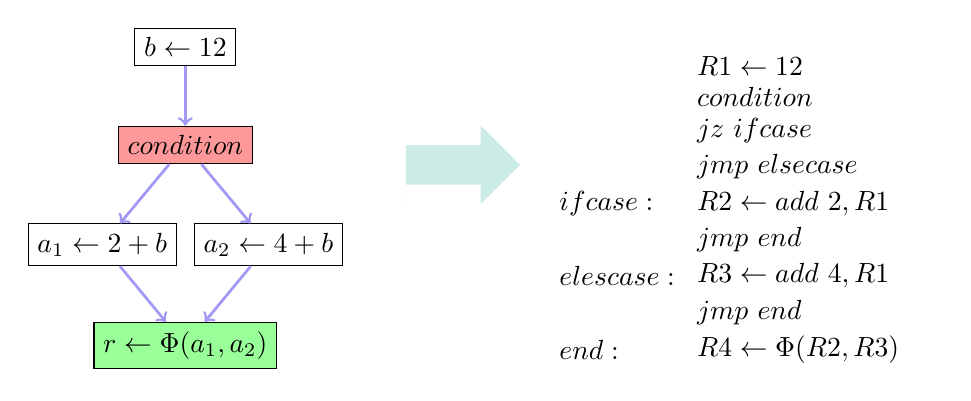
\begin{tikzpicture}
% Graph
\node [cfn,anchor=south] at (2,2)				(ass)		{ $b \leftarrow 12$ };
\node [cfn,cond,below=0.75cm of ass]				(cond)		{ $condition$ };

\node [cfn,below left=0.75cm and -0.75cm of cond]		(left)		{ $a_1 \leftarrow 2 + b$ };
\node [cfn,below right=0.75cm and -0.75cm of cond]		(right)		{ $a_2 \leftarrow 4 + b$ };

\node [cfn,phi,below=2cm of cond]				(phi)		{ $r \leftarrow \Phi(a_1, a_2)$ };


\draw[->,cf]	(ass) to (cond);
\draw[->,cf]	(cond) to (left);
\draw[->,cf]	(cond) to (right);
\draw[->,cf]	(left) to (phi);
\draw[->,cf]	(right) to (phi);



\visible<2-> {
% Arrow
\fill [kit!20] (4.8,0.25) -- (4.8,0.5) -- (5.75,0.5) -- (5.75,0.25) -- (6.25,0.75) -- (5.75,1.25) -- (5.75,1) -- (4.8,1) -- cycle;

% Assembler
\node [ass]	at (10,2)					(aass)		{ $R1 \leftarrow 12$ };
\node [ass,below=-0.1cm of aass]				(acond)		{ $condition$ };
\node [ass,below=-0.1cm of acond]				(acondjmp1)	{ $jz\ ifcase$ };
\node [ass,below=-0.1cm of acondjmp1]				(acondjmp2)	{ $jmp\ elsecase$ };
\node [ass,below=-0.1cm of acondjmp2]				(ifass)		{ $R2 \leftarrow add\ 2, R1$ };
\node [ass,below=-0.1cm of ifass]				(ifjmp)		{ $jmp\ end$ };
\node [ass,below=-0.1cm of ifjmp]				(elseass)	{ $R3 \leftarrow add\ 4, R1$ };
\node [ass,below=-0.1cm of elseass]				(elsejmp)	{ $jmp\ end$ };
\node [ass,below=-0.1cm of elsejmp]				(endnode)	{ $R4 \leftarrow \Phi(R2, R3)$ };

\node [asslabel,left=0 of ifass]				(iflabel)	{$ifcase:$};
\node [asslabel,left=0 of elseass]				(elselabel)	{$elescase:$};
\node [asslabel,left=0 of endnode]				(endlabel)	{$end:$};

}
\end{tikzpicture}

\visible<3-> {
Challenges:
}
\begin{itemize}
\visible<3-> { \item Firm nodes not extendable in jFirm }
\visible<4-> { \item Two operand code in x86 64 assembler:\\
$R2 \leftarrow add 2, R1$ $\Rightarrow$ $mov\ R1, R2$; $add\ 2, R2$ }
\visible<5-> { \item Register allocation }
\end{itemize}
\end{frame}


\begin{frame}
  \frametitle{Register Allocation: Linear Scan}

\begin{itemize}
\item Precondition: Linear register code
\visible<5-> { \item Result: Mapping of Registers to Hardware-Registers }
\end{itemize}

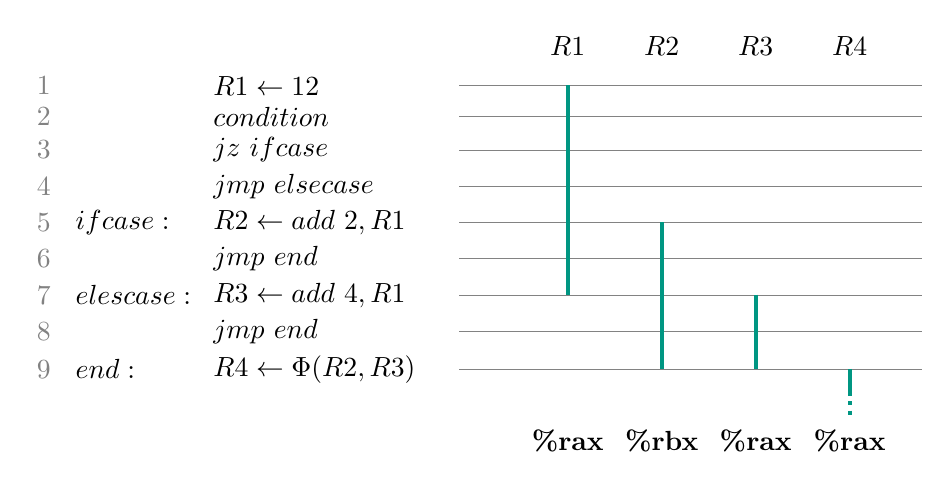
\begin{tikzpicture}
\visible<2-> {
	\node [ass]	at (10,2)					(aass)		{ $R1 \leftarrow 12$ };
\node [ass,below=-0.1cm of aass]				(acond)		{ $condition$ };
\node [ass,below=-0.1cm of acond]				(acondjmp1)	{ $jz\ ifcase$ };
\node [ass,below=-0.1cm of acondjmp1]				(acondjmp2)	{ $jmp\ elsecase$ };
\node [ass,below=-0.1cm of acondjmp2]				(ifass)		{ $R2 \leftarrow add\ 2, R1$ };
\node [ass,below=-0.1cm of ifass]				(ifjmp)		{ $jmp\ end$ };
\node [ass,below=-0.1cm of ifjmp]				(elseass)	{ $R3 \leftarrow add\ 4, R1$ };
\node [ass,below=-0.1cm of elseass]				(elsejmp)	{ $jmp\ end$ };
\node [ass,below=-0.1cm of elsejmp]				(endnode)	{ $R4 \leftarrow \Phi(R2, R3)$ };

\node [asslabel,left=0 of ifass]				(iflabel)	{$ifcase:$};
\node [asslabel,left=0 of elseass]				(elselabel)	{$elescase:$};
\node [asslabel,left=0 of endnode]				(endlabel)	{$end:$};

	\node [assline,left=1.7cm of aass]				(laass)		{ 1 };
\node [assline,left=1.7cm of acond]				(lacond)	{ 2 };
\node [assline,left=1.7cm of acondjmp1]			(lacondjmp1)	{ 3 };
\node [assline,left=1.7cm of acondjmp2]			(lacondjmp2)	{ 4 };
\node [assline,left=1.7cm of ifass]				(lifass)	{ 5 };
\node [assline,left=1.7cm of ifjmp]				(lifjmp)	{ 6 };
\node [assline,left=1.7cm of elseass]				(lelseass)	{ 7 };
\node [assline,left=1.7cm of elsejmp]				(lelsejmp)	{ 8 };
\node [assline,left=1.7cm of endnode]				(lendnode)	{ 9 };

}

\visible<3-> {
	\node []	at (13,2.5)				(reg1)		{ $R1$ };
\node [right=5mm of reg1]				(reg2)		{ $R2$ };
\node [right=5mm of reg2]				(reg3)		{ $R3$ };
\node [right=5mm of reg3]				(reg4)		{ $R4$ };


}

\visible<4-> {
	
\draw[helplinegrey] (aass)		-- ++ (7.5cm, 0);
\draw[helplinegrey] (acond)		-- ++ (7.5cm, 0);
\draw[helplinegrey] (acondjmp1)	-- ++ (7.5cm, 0);
\draw[helplinegrey] (acondjmp2)	-- ++ (7.5cm, 0);
\draw[helplinegrey] (ifass)		-- ++ (7.5cm, 0);
\draw[helplinegrey] (ifjmp)		-- ++ (7.5cm, 0);
\draw[helplinegrey] (elseass)		-- ++ (7.5cm, 0);
\draw[helplinegrey] (elsejmp)		-- ++ (7.5cm, 0);
\draw[helplinegrey] (endnode)		-- ++ (7.5cm, 0);

\draw[reglifetime] ($(reg1.south)+(0,-0.25)$) -- ++ ($(elseass.west)-(aass.west)$);
\draw[reglifetime] ($(reg2.south)+(0,-0.25)-(aass.west)+(ifass.west)$) -- ++ ($(endnode.west)-(ifass.west)$);
\draw[reglifetime] ($(reg3.south)+(0,-0.25)-(aass.west)+(elseass.west)$) --	++ ($(endnode.west)-(elseass.west)$);
\draw[reglifetime] ($(reg4.south)+(0,-0.25)-(aass.west)+(endnode.west)$) -- ++ (0,-0.3);
\draw[reglifetime,dotted] ($(reg4.south)+(0,-0.25)-(aass.west)+(endnode.west)-(0,0.29)$) -- ++ (0,-0.3);


}

\visible<5-> {
\node[resultregister,below=4.5cm of reg1] () { \textbf{\%rax} };
\node[resultregister,below=4.5cm of reg2] () { \textbf{\%rbx} };
\node[resultregister,below=4.5cm of reg3] () { \textbf{\%rax} };
\node[resultregister,below=4.5cm of reg4] () { \textbf{\%rax} };
}

\end{tikzpicture}

\end{frame}


\begin{frame}
  \frametitle{Linear Scan: Extension Graph Coloring}

\begin{tikzpicture}
	\node []	at (13,2.5)				(reg1)		{ $R1$ };
\node [right=5mm of reg1]				(reg2)		{ $R2$ };
\node [right=5mm of reg2]				(reg3)		{ $R3$ };
\node [right=5mm of reg3]				(reg4)		{ $R4$ };


	
\draw[helplinegrey] (aass)		-- ++ (7.5cm, 0);
\draw[helplinegrey] (acond)		-- ++ (7.5cm, 0);
\draw[helplinegrey] (acondjmp1)	-- ++ (7.5cm, 0);
\draw[helplinegrey] (acondjmp2)	-- ++ (7.5cm, 0);
\draw[helplinegrey] (ifass)		-- ++ (7.5cm, 0);
\draw[helplinegrey] (ifjmp)		-- ++ (7.5cm, 0);
\draw[helplinegrey] (elseass)		-- ++ (7.5cm, 0);
\draw[helplinegrey] (elsejmp)		-- ++ (7.5cm, 0);
\draw[helplinegrey] (endnode)		-- ++ (7.5cm, 0);

\draw[reglifetime] ($(reg1.south)+(0,-0.25)$) -- ++ ($(elseass.west)-(aass.west)$);
\draw[reglifetime] ($(reg2.south)+(0,-0.25)-(aass.west)+(ifass.west)$) -- ++ ($(endnode.west)-(ifass.west)$);
\draw[reglifetime] ($(reg3.south)+(0,-0.25)-(aass.west)+(elseass.west)$) --	++ ($(endnode.west)-(elseass.west)$);
\draw[reglifetime] ($(reg4.south)+(0,-0.25)-(aass.west)+(endnode.west)$) -- ++ (0,-0.3);
\draw[reglifetime,dotted] ($(reg4.south)+(0,-0.25)-(aass.west)+(endnode.west)-(0,0.29)$) -- ++ (0,-0.3);


\visible<2-3> {
	\node[graphnode,below right=0.5cm and 2cm of reg4]	(graphr1)	{ $R1$ };
	\node[graphnode,right=2cm of graphr1]			(graphr2)	{ $R2$ };
	\node[graphnode,below=2cm of graphr1]			(graphr3)	{ $R3$ };
	\node[graphnode,right=2cm of graphr3]			(graphr4)	{ $R4$ };
}
\visible<4-> {
	\node[graphnode,fill=kit!40,below right=0.5cm and 2cm of reg4]	(graphr1)	{ $R1$ };
	\node[graphnode,fill=kitblue!40,right=2cm of graphr1]			(graphr2)	{ $R2$ };
	\node[graphnode,fill=kit!40,below=2cm of graphr1]			(graphr3)	{ $R3$ };
	\node[graphnode,fill=kit!40,right=2cm of graphr3]			(graphr4)	{ $R4$ };
}

\visible<3-> {
	\draw (graphr1) -- (graphr2);
	\draw (graphr3) -- (graphr2);
}

\visible<5-> {
\node[colorbox,fill=kit!40,below=0.5cm of graphr3] (color1)	{ };
\node[colorbox,fill=kitblue!40,below=0.2cm of color1] (color2)	{ };

\node[right=0.5cm of color1] () { \textbf{\%rax} };
\node[right=0.5cm of color2] () { \textbf{\%rbx} };
}

\end{tikzpicture}

\end{frame}

\begin{frame}
  \frametitle{SSA-Based Register Allocation}

\begin{center}
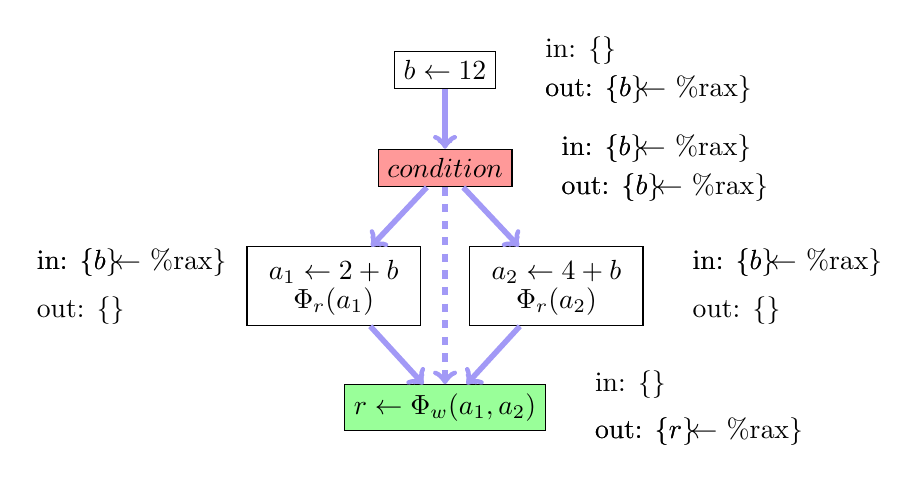
\begin{tikzpicture}
% Graph
\node [cfn,anchor=south] at (2,2)				(ass)		{ $b \leftarrow 12$ };
\node [cfn,cond,below=0.75cm of ass]				(cond)		{ $condition$ };

\node [cfn,below left=0.75cm and -0.55cm of cond,minimum height=10mm,minimum width=22mm]	(left)		{  };
\node [above=-6mm of left]					(leftc)		{ $a_1 \leftarrow 2 + b$ };
\node [below=-2mm of leftc]					(leftphi)	{ $\Phi_r(a_1)$ };

\node [cfn,below right=0.75cm and -0.55cm of cond,minimum height=10mm,minimum width=22mm]	(right)		{  };
\node [above=-6mm of right]					(rightc)	{ $a_2 \leftarrow 4 + b$ };
\node [below=-2mm of rightc]					(rightphi)	{ $\Phi_r(a_2)$ };

\node [cfn,phi,below=2.5cm of cond]				(phi)		{ $r \leftarrow \Phi_w(a_1, a_2)$ };


\draw[->,cf]	(ass) to (cond);
\draw[->,cf]	(cond) to (left);
\draw[->,cf]	(cond) to (right);
\draw[->,cf]	(left) to (phi);
\draw[->,cf]	(right) to (phi);



\visible<2-> {\node[above right=-3mm and 5mm of ass]	(ass-life-in) {in: \{\} }; }
\visible<2> {\node[below right=-3mm and 5mm of ass]	(ass-life-out) 		{out: \{$b$\} };}
\visible<3-> {\node[below right=-3mm and 5mm of ass]	(ass-life-out) 		{out: \{$b \leftarrow$ \%rax\} };}

\visible<2> {\node[above right=-3mm and 5mm of cond]	(cond-life-in) 		{in: \{$b$\} };}
\visible<3-> {\node[above right=-3mm and 5mm of cond]	(cond-life-in)		{in: \{$b \leftarrow$ \%rax\} };}
\visible<2> {\node[below right=-3mm and 5mm of cond]	(cond-life-out) 	{out: \{$b$\} };}
\visible<3-> {\node[below right=-3mm and 5mm of cond]	(cond-life-out) 	{out: \{$b \leftarrow$ \%rax\} };}

\visible<2> {\node[above right=-5mm and -50mm of left]	(left-life-in) 	{in: \{$b$\} };}
\visible<3-> {\node[above right=-5mm and -50mm of left]	(left-life-in) 	{in: \{$b \leftarrow$ \%rax\} };}
\visible<2-> {\node[below right=-5mm and -50mm of left]	(left-life-out) 	{out: \{\} }; }

\visible<2> {\node[above right=-5mm and 5mm of right]	(right-life-in) 	{in: \{$b$\} };}
\visible<3-> {\node[above right=-5mm and 5mm of right]	(right-life-in) 	{in: \{$b \leftarrow$ \%rax\} };}
\visible<2-> { \node[below right=-5mm and 5mm of right]	(right-life-out) 	{out: \{\} }; }

\visible<2-> { \node[above right=-3mm and 5mm of phi]	(phi-life-in) 		{in: \{\} }; }
\visible<2-6> {\node[below right=-3mm and 5mm of phi]	(phi-life-out) 		{out: \{$r$\} };}
\visible<7-> {\node[below right=-3mm and 5mm of phi]	(phi-life-out) 		{out: \{$r \leftarrow$ \%rax\} };}

\visible<3-> { \draw[->,cfb]	(ass) to (cond); }
\visible<4-> { \draw[->,cfb]	(cond) to (left); }
\visible<5-> { \draw[->,cfb]	(cond) to (right); }
\visible<6-> {
	\draw[->,cfb,dashed]	(cond) to (phi);
	\draw[->,cfb]	(left) to (phi);
	\draw[->,cfb]	(right) to (phi);
}



\end{tikzpicture}
\end{center}
\end{frame}

\begin{frame}
  \frametitle{Block Ordering}
\end{frame}

\begin{frame}
  \frametitle{Conclusion}


\begin{itemize}
	\item Firm makes (good) work!
	\begin{itemize}
		\item Especially with Windows
	\end{itemize}
	\item Testing is important
	\item GIT is nice, but its usage can be tricky for beginners
\end{itemize}

\visible<2> {
\begin{figure}

\includegraphics[width=0.25\textwidth]{images/egg.jpg}
\caption{ Source: www.real-drive.de }
\label{fig:harps_example}
\end{figure}
}
\end{frame}

\begin{frame}
  \frametitle{Implemented Optimizations}
\end{frame}

\begin{frame}
  \frametitle{Facts and Numbers}
\end{frame}

\end{document}
